\chapter{Tecnologias Utilizadas}
\label{chap3}

\section{Neo4j}
O Neo4j é um banco de dados NoSQL orientado a grafos, que opera sob uma estrutura de dados que consiste em nós, relacionamentos e propriedades. Ao contrário dos bancos de dados relacionais, que usam tabelas e linhas, o Neo4j permite que as informações sejam armazenadas em um formato altamente conectado, imitando as interações do mundo real. Isso faz do Neo4j uma escolha ideal para cenários onde as relações entre os dados são tão importantes quanto os próprios dados.

O Neo4j é um sistema de gerenciamento de banco de dados orientado a grafos desenvolvido pela Neo4j Inc. Seus elementos de dados consiste em nós, relacionamentos e propriedades. Ao contrário dos bancos de dados relacionais, que usam tabelas e linhas
Cada Nó e cada Aresta possui um ou mais “Label”s (Rótulos), que definem o tipo do dado e instanciam um index de lookup, funcionando similar à uma tabela num banco SQL.

Cada label possui sua definição com suas propriedades, incluindo possíveis arestas e ligações com nós de outras labels. Tais definições de tipos são determinada seguindo a sintaxe da biblioteca @neo4j/graphql, onde escrevemos e documentamo-os, e são utilizados para gerar o Schema do Banco de Dados.


\subsection{Cypher Query Language}

O banco Neo4j, diferentemente da maioria dos bancos relacionais, não utiliza SQL como a linguagem de manipulação de registros de dados, e sim a própria linguagem chamada Cypher.

\begin{figure}[H]
    \centering
    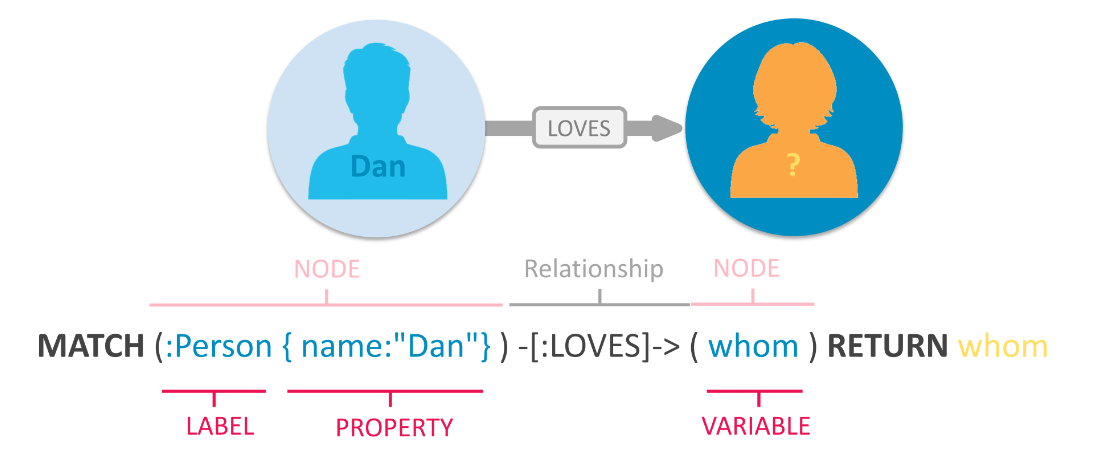
\includegraphics[width=1.0\linewidth]{Imagens/chap03/cypher-exemple.png}
    \caption{Exemplo Cypher https://neo4j.com/developer/cypher/.}
    \label{fig:profile-exemple}
\end{figure}
https://neo4j.com/developer/cypher/

\section{GraphQL}


\subsection{@neo4j/graphql}
A GraphQL to Cypher query execution layer for Neo4j and JavaScript GraphQL implementations.

Para realizar a conexão entre as requisições em GraphQL que a interface do usuário irá realizar com o banco de dados, precisamos realizar essa tradução para a Cypher Query Language que será executada no banco. Para tal trabalho a neo4j disponibiliza uma biblioteca que permite tanto definir e gerar o schema do banco de dados, como gerar automaticamente requisições de CRUD para cada um dos \textit{tipos} definidos.

\section{Apollo}

\section{Node.js}

\subsection{Express.js}

\section{Vue.js}
